\section{Introduction}

Ionic Polymer-Metal Composites (IPMC) have been studied during the past two 
decades for their potential to serve as noiseless mechanoelectrical and electromechanical 
transducers \cites{basu1997membrane,shahinpoor2001smartmat,
nasser2002applied,newbury2003intelligent, wallmersperger2007appliedphysics,
pugal2008appliedphysics,pugal2010polymer}.
The advantages of IPMC over other electroactive polymer actuators
are low voltage bending, high strains ($>1\%$), and an ability to work
in wet environments. A typical IPMC consists of a thin sheet of polymer
(often Nafion or Teflon) which is sandwiched between noble
metal electrodes such as platinum or gold. When fabricated, the polymer 
membrane is saturated with certain solvent and ions such as water and $H^+$.
When a voltage is applied to the electrodes, the counter ions start
migrating due to the imposed electric field. By dragging along the solvent,
the osmotic pressure difference near the electrodes
results in bending of the material (see Fig.~\ref{fig:conceptual}).
\begin{figure}[!ht]
  \begin{centering}
  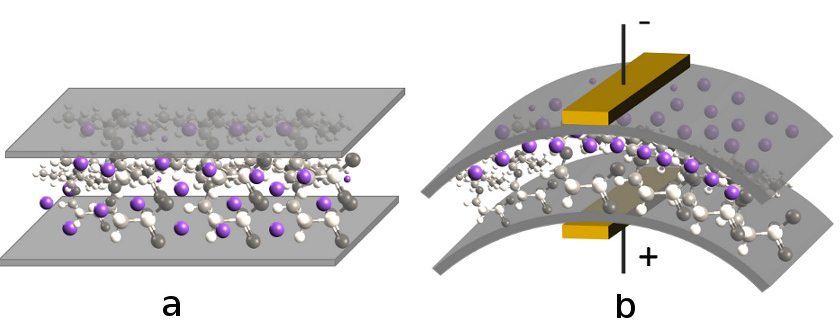
\includegraphics[scale=0.7]{IPMC_bending}
  \caption{\label{fig:conceptual}Conceptual model of the actuation
 	of IPMC. Initial counter ion distribution (a) and
	the distribution and resulting bending after applying a voltage (b).}
  \end{centering}
%\vspace{-1cm}
\end{figure}
%\newpage

In this study we will model IPMC materials via a multiphysics coupled problem 
consisting of the Poisson and Nernst-Planck equations (abbreviated by PNP in
the following). These equations are used to model charge transport in materials 
that include ionic migration, diffusion, and convection. The charge transport 
process is a key mechanism for electromechanical transduction.

The PNP system is highly nonlinear and for a typical domain with two
electrodes, largest differences in charge concentration occur in a very narrow
region near the boundary. The computing power required for a full scale problem 
is significant~\cite{pugal2010spie3d}. This is why we are interested in exploring adaptive algorithms
-- we hope to obtain meshes that are optimal in terms of calculation time and 
calculation error.

The Nernst-Planck equation for a mobile species ---
in our case for counter ions --- has the form
\begin{equation}
  \frac{\partial C}{\partial t}+\nabla\cdot(-D\nabla C-\mu FC\nabla\phi)=0.
  \label{eq:nernst-planck}
\end{equation}
Here $C$ stands for the counter ion concentration with the initial value of $C_0$,
$D$ is diffusion, $\mu$ mobility,
$F$ Faraday constant, and $\phi$ voltage. We have neglected 
the velocity of the species as in our case it can be assumed zero. 
The Poisson equation has the form
\begin{equation}
  -\nabla^2\phi=\frac{F\rho}{\varepsilon}
  \label{eq:poisson}
\end{equation}
where $\varepsilon$ is the absolute dielectric permittivity. The
charge density $\rho = C-C_{0}$ 
where $C_{0}$ is a constant anion concentration.

The outline of the paper is as follows: Section \ref{sec:moti} shows that 
the solution components $C$ and $\phi$ have very different behavior, which
is the reason why it is difficult to find a common mesh that would be optimal 
for both of them. This explains why we are interested in approximation them
on individual meshes equipped with mutually independent adaptivity 
mechanisms. The PNP model is presented in Section~\ref{sec:model} where also its weak 
formulation for the Newton's method is derived. Section~\ref{sec:hermes}
presents a brief overview of a novel adaptive multi-mesh $hp$-FEM 
method~\cite{solin2010monolithic,solin2010adaptive,dubcova2010space,solini2010adaptive}
that is used to solve the 
problem numerically. Numerical results and comparisons are presented in Section~\ref{sec:results}, 
and conclusion and outlook are drawn in Section~\ref{sec:conc}.


